
\documentclass{article}

\usepackage{modified_dscproblemset}
\usepackage[margin=0.7in]{geometry}
\usepackage{amsmath}
\usepackage{amssymb}
\usepackage{booktabs}
\usepackage{nicefrac}
\usepackage{tikz}
\usepackage{pgfplots}
\usepackage{url}
\usepackage{multicol}
\usepackage{scrextend}
\usepackage{graphbox,graphicx}
\usepackage[outputdir=build]{minted}
\usepackage{gensymb, comment}
\usepackage{bm}

\usetikzlibrary{positioning}

\newcommand{\avocado}{%
  \begingroup\normalfont
  \includegraphics[height=2\fontcharht\font`\B, align=c]{pics/avo.png}%
  \endgroup
}

\newcommand{\avo}[1]{\multido{}{#1}{\avocado}\hspace{0.2em}}


% this controls whether solutions are shown or not
    \showsolntrue

% commands
% ------------------------------------------------------------------------------

\newcommand{\python}[1]{\mintinline{python}{#1}}

% ------------------------------------------------------------------------------

\begin{document}

\pstitle{%
    Midterm Exam%
}{DSC 40A, Fall 2021}
\vspace{1em}

\hline

\vspace{.15in}

\textbf{Instructions}

\begin{itemize}
    \item This exam consists of 5 questions (including Question 0), worth a total of 36 points. \textbf{Advice: Read all of the problems before starting to work.}
    \item This exam must be completed and submitted to Gradescope in the 90 minute period ending at 12:30 PM PST.
    \item \textbf{This exam is open-book and open-Internet, but collaboration is strictly forbidden.}
    \item Show your work for all questions. Correct answers with no work shown may not receive full credit.
    \item Please write or type neatly.
\end{itemize}

\vspace{.15in}

\hline

\vspace{.3in}

\textbf{0. Statement of Academic Integrity}[1 Point]

Please copy, sign, and date the following statement on your exam page. You must do this even if you are doing the exam on a separate piece of paper. \textbf{Your exam will not be graded if you do not complete this question.}

\textit{As a member of the UC San Diego community, I act with honesty, integrity, and respect for others. I will neither give nor receive assistance while taking this exam.}


\newpage
\begin{probset}

\vspace{.25in}

\begin{prob}[\textbf{Instagram Chronicles}][9 Points]

King Triton just made an Instagram account and has been keeping track of the number of likes his posts have received so far.

His first 7 posts have received a mean of 16 likes; the specific like counts in sorted order are

$$8, 12, 12, 15, 18, 20, 27$$

King Triton wants to predict the number of likes his next post will receive, using a constant prediction rule $h$. For each loss function $L(h, y)$, determine the constant prediction $h^*$ that minimizes empirical risk. If you believe there are multiplie minimizers, specify them all. If you believe you need more information to answer the question or that there is no minimizer, state that clearly. \textbf{Give a brief justification for each answer.}

\begin{subprobset}

\begin{subprob}[1 Point]
$L(h, y) = |y - h|$

\begin{soln}
\textbf{15}. This is squared loss, and hence we're looking for the minimizer of mean absolute error, which is the median, 15.
\end{soln}
\end{subprob}

\vspace{.75in}

\begin{subprob}[1 Point]
$L(h, y) = (y - h)^2$

\begin{soln}
\textbf{16}. This is squared loss, and hence we're looking for the minimizer of mean squared error, which is the mean, 16.
\end{soln}
\end{subprob}

\vspace{.75in}

\begin{subprob}[1.5 Points]
$L(h, y) = 4(y - h)^2$

\begin{soln}
\textbf{16}. This is squared loss, multiplied by a constant. Note that when we go to minimize empirical risk for this loss function, we will take the derivative of empirical risk and set it equal to 0; at that point the constant factor of 4 can be divided from both sides, so this problem boils down to minimizing ordinary mean squared error. The only difference is that the graph of mean squared error will be stretched vertically by a factor of 4; the minimizing value will be in the same place.

For more justification, here we consider any general re-scaling $\alpha (y-h)^2$:

\begin{align*}
    R_{sq}(h) &= \frac{1}{n} \sum_{i = 1}^n \alpha (y_i - h)^2 \\
              &= \alpha \cdot \frac{1}{n} \sum_{i = 1}^n (y_i - h)^2 \\
  \frac{d}{dh} R_{sq}(h) &= \alpha \cdot \frac{1}{n} \sum_{i = 1}^n 2(y_i - h)(-1) = 0\\
  &\implies -\frac{2\alpha}{n}\sum_{i = 1}^n (y_i - h) = 0 \\
  &\implies \sum_{i = 1}^n (y_i - h) = 0 \\
  &\implies h^* = \frac{1}{n} \sum_{i = 1}^n y_i
\end{align*}

\end{soln}
\end{subprob}

\vspace{.75in}

\begin{subprob}[1.5 Points]
$L(h, y) = \begin{cases} 0 & h = y \\ 100 & h \neq y \end{cases}$

\begin{soln}
\textbf{12}.

This is a scaled version of 0-1 loss. We know that empirical risk for 0-1 loss is minimized at the mode, so that also applies here. The mode, i.e. the most common value, is 12.

\end{soln}
\end{subprob}

\vspace{.75in}

\begin{subprob}[2.5 Points]
$L(h, y) = (3y - 4h)^2$

\begin{soln}
\textbf{12}.

Note that we can write $(3y - 4h)^2$ as $\left( 3 \left( y - \frac{4}{3}h \right) \right)^2 = 9 \left( y - \frac{4}{3}h \right)^2$. As we've seen, the constant factor out front has no impact on the minimizing value. Using the same principle as in the last part, we can say that $$\frac{4}{3} h^* = \bar{x} \implies h^* = \frac{3}{4} \bar{x} = \frac{3}{4} \cdot 16 = 12$$

\end{soln}
\end{subprob}

\vspace{1in}

\begin{subprob}[1.5 Points]
$L(h, y) = (y - h)^3$

\textit{Hint: Do not spend too long on this subpart.}

\begin{soln}
\textbf{No minimizer}.

Note that unlike $|y - h|$, $(y - h)^2$, and all of the other loss functions we've seen, $(y - h)^3$ tends towards $-\infty$, rather than having a minimum output of 0. This means that there is no $h$ that minimizes $\frac{1}{n} \sum_{i = 1}^n (y_i - h)^3$; the larger we make $h$, the more negative (and hence ``smaller") this empirical risk becomes.

\end{soln}
\end{subprob}

\vspace{.75in}

\end{subprobset}

\end{prob}

\newpage

\begin{prob}[\textbf{Seeing Double}][9 Points]

Consider a set of 23 data points $y_1, y_2, y_3, ..., y_{23}$ such that $y_1 < y_2 < ... < y_{23}$. Let's call this Dataset A.

We create a new dataset, Dataset B, by repeating each point in Dataset A once. That is, Dataset B is the set of 46 points $y_1, y_1, y_2, y_2, ..., y_{23}, y_{23}$.

Answer the following questions regarding the relationship between Dataset A and Dataset B. \textbf{Justify your answers.}

\begin{subprobset}

\begin{subprob}[3 Points]
Suppose the minimizer of mean absolute error $R_{abs}(h)$ for Dataset A is 5. What is the minimizer of mean absolute error for Dataset B? If you believe there are multiple minimizers, specify them all. If you believe you need more information to answer the question, state that clearly.

\begin{soln}

The minimizer of MAE for Dataset B is still 5. Note that when we repeat each data point, we go from having an odd number of data points (23) to an even number (46). This means the minimizer is the set of all values between the middle two values. But the middle two values will now both be $y_{12}$, and so there are no numbers ``in between" them -- only $y_{12}$ minimizes MAE.

\end{soln}

\end{subprob}

\vspace{1.5in}

\begin{subprob}[3 Points]
Suppose the \textit{mean absolute deviation from the median} for Dataset A is 17. What is the \textit{mean absolute deviation from the median} for Dataset B? If you believe you need more information to answer the question, state that clearly.

\begin{soln}

The mean absolute deviation from the median for Dataset B is still 17. As we saw in part a, the median itself does not change. When adding together the deviations from the median, each point is repeated twice, so the sum of all deviations from the median is doubled. However, there are twice as many data points in Dataset B than there are in Dataset A, so we divide by $2n$ (46) instead of $n$ (23) in our average. 

In short, for Dataset B both the numerator and denominator in the calculation of mean absolute deviation from the median $\frac{\sum_{i = 1}^n |y_i - \text{Median}(y)|}{n}$ are double what they were for Dataset A, so the end result is the same as for Dataset A.

\end{soln}

\end{subprob}

\vspace{1.55in}

\begin{subprob}[3 Points]
Suppose the function $R_A(h)$ represents mean absolute error for Dataset A and $R_B(h)$ represents mean absolute error for Dataset B.

Is it true that $R_A(h) = R_B(h)$ for any real number $h$? (In other words, are the graphs of $R_A(h)$ and $R_B(h)$ identical?) Explain your reasoning.

\begin{soln}

Yes they are.

Recall that the definition of $R_{abs}(h)$ is

$$R_{abs}(h) = \frac{1}{n} \sum_{i = 1}^n |y_i - h|$$

For the first dataset, we have

$$R_{A}(h) = \frac{1}{23} \sum_{i = 1}^{23} |y_i - h|$$

and for the second dataset, we have

\begin{align*}R_{B}(h) &= \frac{1}{46} \sum_{i = 1}^{46} \left( |y_1 - h| + |y_1 - h| + |y_2 - h| + |y_2 - h| + ... + |y_{23} - h| + |y_{23} - h| \right) \\
&= \frac{1}{46} \left( 2 \sum_{i = 1}^{23} |y_i - h| \right) \\ &= \frac{1}{23} \sum_{i = 1}^{23} |y_i - h| \\ &= R_{A}(h) \end{align*}


\end{soln}

\vspace{1in}

\end{subprob}

\end{subprobset}

\end{prob}

\newpage

\begin{prob}[\textbf{Descending Gradiently}][8 Points]

Remember to show your work and justify your answers.

Suppose we want to minimize the function

$$R(h) = e^{(h + 1)^2}$$

\begin{subprobset}

\begin{subprob}[1.5 Points]
Without using gradient descent or calculus, what is the value $h^*$ that minimizes $R(h)$?

\begin{soln}

The minimum possible value of the exponent is $0$, since anything squared is non-negative. The exponent is 0 when $(x+1)^2 = 0$, i.e. when $x = -1$. Since $e^{(x+1)^2}$ gets larger as $(x+1)^2$ gets larger, the minimizing input $h^*$ is $-1$.

\end{soln}

\end{subprob}

\vspace{1in}

\begin{subprob}[4 Points]
Now, suppose we want to use gradient descent to minimize $R(h)$. Assume we use an initial guess of $h_0 = 0$. What is $h_1$? Give your answer in terms of a generic step size, $\alpha$, and other constants. ($e$ is a constant.)

\begin{soln}

First, we find $\frac{dR}{dh}(h)$:

$$\frac{dR}{dh}(h) = 2(x+1) e^{(x+1)^2}$$

Then, we know that

$$h_1 = h_0 - \alpha \frac{dR}{dh}(h_0) = 0 - \alpha \frac{dR}{dh}(0)$$

In our case, $\frac{dR}{dh}(0) = 2(0 + 1) e^{(0+1)^2} = 2e$, so

$$h_1 = -\alpha \cdot 2e$$

\end{soln}

\end{subprob}

\vspace{1.75in}

\begin{subprob}[1.5 Point]
Using your answers from the previous two parts, what should we set the value of $\alpha$ to be if we want to ensure that gradient descent finds $h^*$ after just one iteration?

\begin{soln}

We know from part b that $h_1 = -\alpha \cdot 2e$, and we know from part a that $h^* = -1$. If gradient descent converges in one iteration, that means that $h_1 = h^*$; solving this yields

$$-\alpha \cdot 2e = -1 \implies \alpha = \frac{1}{2e}$$

\end{soln}

\end{subprob}

\vspace{1.25in}

\begin{subprob}[1 Point]
Below is a graph of $R(h)$ with no axis labels.
\begin{center}
    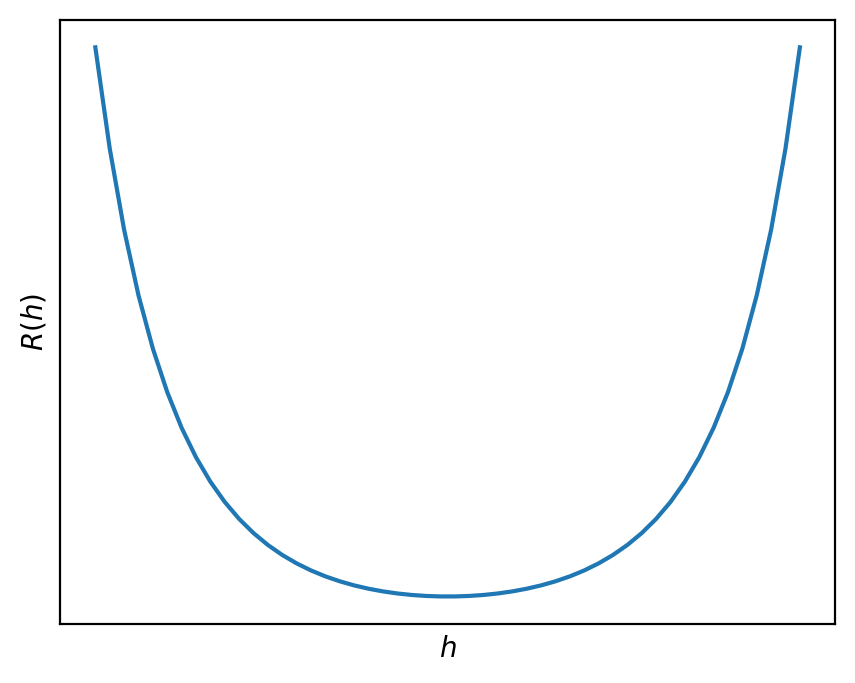
\includegraphics[width=2in]{pics/midterm/grad-desc.png}
\end{center}

True or False: Given an appropriate choice of step size, $\alpha$, gradient descent is guaranteed to find the minimizer of $R(h)$.

\begin{soln}
\textbf{True}. $R(h)$ is convex, since the graph is bowl shaped. (It can also be proved that $R(h)$ is convex using the second derivative test.) It is also differentiable, as we saw in part (b). As a result, since it's both convex and differentiable, gradient descent is guaranteed to be able to minimize it given an appropriate choice of step size.
\end{soln}

\vspace{.85in}

\end{subprob}

\end{subprobset}

\end{prob}

\newpage

\begin{prob}[\textbf{Dirty Bird Gets The Worm}][9 Points]

Billy, the avocado farmer from Homework 3, wasn't making enough money growing avocados and decided to take on a part-time job as a waiter at the restaurant Dirty Birds on campus. For two months, he kept track of all of the total bills he gave out to customers along with the tips they then gave him, all in dollars. Below is a scatter plot of Billy's tips and total bills.

\begin{center}
    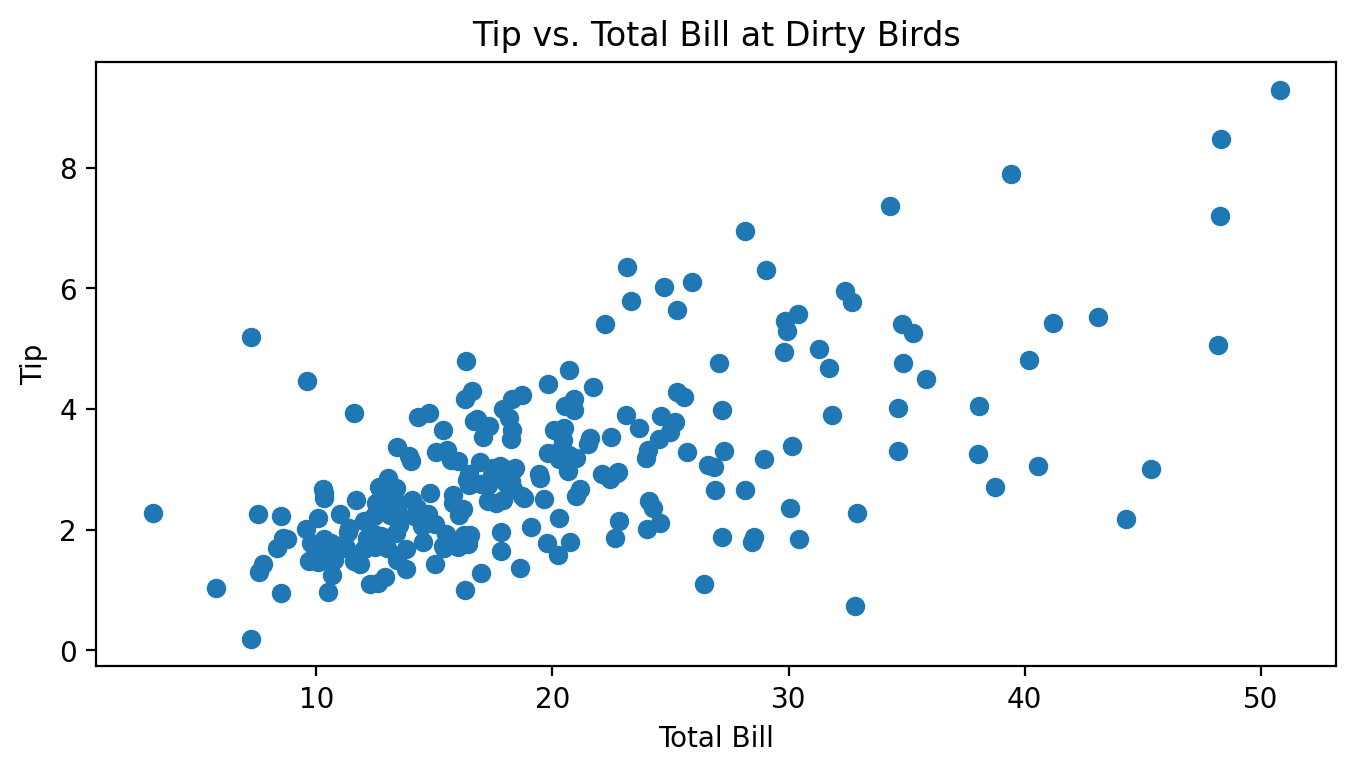
\includegraphics[width=3in]{pics/midterm/dirtybirds.png}
\end{center}

Throughout this question, assume we are trying to fit a linear prediction rule $H(x) = w_0 + w_1x$ that uses total bills to predict tips, and assume we are finding optimal parameters by minimizing mean squared error.

\begin{subprobset}

\begin{subprob}[2 Points]
Which of these is the most likely value for $r$, the correlation between total bill and tips? Why?

\begin{center}
    $$-1 \qquoad -0.75 \qquad -0.25 \qquad 0 \qquad 0.25 \qquad 0.75 \qquad 1$$
\end{center}

\begin{soln}
0.75. It seems like there is a pretty strong, but not perfect, linear association between total bills and tips.

\end{soln}

\vspace{.65in}

\end{subprob}

\begin{subprob}[3 Points]
The variance of the tip amounts is 2.1. Let M be the mean squared error of the best linear prediction rule on this dataset (under squared loss). Is $M$ less than, equal to, or greater than 2.1? How can you tell?

\begin{soln}

$M$ is less than 2.1. The variance is equal to the MSE of the constant prediction rule. 

Note that the MSE of the best linear prediction rule will always be less than or equal to the MSE of the best constant prediction rule $h$. The only case in which these two MSEs are the same is when the best linear prediction rule is a flat line with slope 0, which is the same as a constant prediction. In all other cases, the linear prediction rule will make better predictions and hence have a lower MSE than the constant prediction rule. 

In this case, the best linear prediction rule is clearly not flat, so $M < 2.1$.

\end{soln}

\vspace{1in}

\end{subprob}

\begin{subprob}[4 Points]
Suppose we use the formulas from class on Billy's dataset and calculate the optimal slope $w_1^*$ and intercept $w_0^*$ for this prediction rule.

Suppose we add the value of 1 to every total bill $x$, effectively shifting the scatter plot 1 unit to the right. \textbf{Note that doing this does not change the value of $w_1^*$.} What amount should we add to each tip $y$ so that the value of $w_0^*$ also does not change? Your answer should involve one or more of $\bar{x}, \bar{y}, w_0^*, w_1^*,$ and any constants.

\textit{Note: To receive full points, you must provide a rigorous explanation, though this explanation only takes a few lines. However, we will award partial credit to solutions with the correct answer, and it's possible to arrive at the correct answer by drawing a picture and thinking intuitively about what happens.}

\begin{soln}

First, we present the rigorous solution.

Let $\bar{x_\text{old}}$ represent the previous mean of the $x$'s and $\bar{x_\text{new}}$ represent the new mean of the $x$'s. Then, we know that $\bar{x_\text{new}} = \bar{x_\text{old}} + 1$.

Also, let $\bar{y_\text{old}}$ and $\bar{_\text{new}}$ represent the old and new mean of the $y$'s. We will try and find a relationship between these two quantities.

We want the two intercepts to be the same. The intercept for the old line is $\bar{y_\text{old}} - w_1^* \bar{x_\text{old}}$ and the intercept for the new line is $\bar{y_\text{new}} - w_1^* \bar{x_\text{new}}$. Setting these equal yields

\begin{align*}
    \bar{y_\text{new}} - w_1^* \bar{x_\text{new}} &= \bar{y_\text{old}} - w_1^* \bar{x_\text{old}} \\
     \bar{y_\text{new}} - w_1^* (\bar{x_\text{old}} + 1) &= \bar{y_\text{old}} - w_1^* \bar{x_\text{old}} \\
     \bar{y_\text{new}} &= \bar{y_\text{old}} - w_1^* \bar{x_\text{old}} + w_1^* (\bar{x_\text{old}} + 1) \\
     \bar{y_{\text{new}}} &= \bar{y_\text{old}} + w_1^*
\end{align*}

Thus, in order for the intercepts to be equal, we need the mean of the new $y$'s to be $w_1^*$ greater than the mean of the old $y$'s. Since we're told we're adding the same constant to each $y$, that constant is $w_1^*$.

\vspace{.2in}

Another way to approach the question is as follows: consider any point that lies directly on a line with slope $w_1^*$ and intercept $w_0^*$. Consider how the slope between two points on a line is calculated: $\text{slope} = \frac{y_2 - y_1}{x_2 - x_1}$. If $x_2 - x_1 = 1$, in order for the slope to remain fixed we must have that $y_2 - y_1 = \text{slope}$. For a concrete example, think of the line $y = 5x + 2$. The point $(1, 7)$ is on the line, as is the point $(1 + 1, 7 + 5) = (2, 12)$.

In our case, none of our points are guaranteed to be \textbf{on} the line defined by slope $w_1^*$ and intercept $w_0^*$. Instead, we just want to be guaranteed that the points have the same regression line after being shifted. If we follow the same principle, though, and add 1 to every $x$ and $w_1^*$ to every $y$, the points' relative positions to the line will not change (i.e. the vertical distance from each point to the line will not change), and so that will remain the line with the lowest MSE, and hence $w_0^*$ and $w_1^*$ won't change.

\end{soln}

\vspace{1in}

\end{subprob}

\end{subprobset}

\end{prob}

\end{probset}

\end{document}
